\documentclass[10pt]{beamer}

\usepackage{mathtools, 
amsmath, 
amssymb, 
amsthm, 
graphicx, 
textcomp, 
enumerate, 
diagbox, 
tcolorbox,
esvect, 
xcolor,
soul, 
tikz, 
utopia, 
adjustbox,
tikz-cd,
quiver}


\usepackage{hyperref}


\usetheme{CambridgeUS}

% \definecolor{myNewColorA}{RGB}{12,12,110}
% \definecolor{myNewColorB}{RGB}{16,85,154}
% \definecolor{myNewColorC}{RGB}{150,158,197}
% \setbeamercolor*{palette primary}{bg=myNewColorC}
% \setbeamercolor*{palette secondary}{bg=myNewColorB, fg = white}
% \setbeamercolor*{palette tertiary}{bg=myNewColorA, fg = white}
% \setbeamercolor*{titlelike}{fg=myNewColorA}
% \setbeamercolor*{title}{bg=myNewColorA, fg = white}
% \setbeamercolor*{item}{fg=myNewColorA}
% \setbeamercolor*{caption name}{fg=myNewColorA}
% \usefonttheme{default}


%%%%%COMMON SETS%%%%%%%%%%%%%%%%%%%%%%%%%%%%%%%%%%%%%%

\newcommand{\Z}{\mathbb{Z}} 
\newcommand{\R}{\mathbb{R}}
\newcommand{\Q}{\mathbb{Q}}
\newcommand{\N}{\mathbb{N}}
\newcommand{\C}{\mathbb{C}}
\newcommand{\F}{\mathbb{F}}
\newcommand{\cI}{\mathcal{I}}



\newcommand{\gen}[1]{\langle#1\rangle} % generated group
\newcommand{\Aut}{\mathrm{Aut}} % automorphism group


% Quandles
\newcommand{\cL}{\mathcal{L}}
\newcommand{\qgen}[1]{\langle\langle#1\rangle\rangle}
\newcommand{\Conj}{\mathrm{Conj}} % conjugate quandle
\newcommand{\sq}{\preccurlyeq} % subquandle
\newcommand{\thru}{\rhd} % through
\newcommand{\bthru}{\inv{\thru}} % backthrough
\newcommand{\Inn}{\mathrm{Inn}} % inner automorphism group
\newcommand{\Trans}{\mathrm{Trans}} % transvection group
\newcommand{\Adconj}{\mathrm{Adconj}} % adconj group
\newcommand{\bigthru}{\scalebox{1.5}{$\rhd$}} % big through
\newcommand{\psq}{\prec} %subquand
\newcommand{\Tak}{\mathrm{Tak}}
\newcommand{\Adtak}{\mathrm{Adtak}}

%%%%%%%%FUNCTIONS%%%%%%%%%%%%%%%%%%%%%%%%
\newcommand{\inv}[1]{#1^{-1}}
\newcommand{\im}{\text{im}} % image


\theoremstyle{plain}
\newtheorem{remark}{Remark}
\newtheorem{proposition}{Proposition}
\newtheorem{claim}{Claim}
\newtheorem{subclaim}{Subclaim}
\newtheorem{tool}{Tool}
\newtheorem{conjecture}{Conjecture}
\newtheorem{question}{Question}



\setbeamerfont{title}{size=\large}
\setbeamerfont{subtitle}{size=\small}
\setbeamerfont{author}{size=\small}
\setbeamerfont{date}{size=\small}
\setbeamerfont{institute}{size=\small}


\AtBeginSection[]{
  \begin{frame}
  \vfill
  \centering
  \begin{beamercolorbox}[sep=8pt,center,shadow=true,rounded=true]{title}
    \usebeamerfont{title}\insertsectionhead\par%
  \end{beamercolorbox}
  \vfill
  \end{frame}
}

\usepackage[backend = biber]{biblatex}
\addbibresource{presentation.bib}

\title{Complementation of Subquandles}
\author{D.N. Yetter, K.J. Amsberry, M.H. Lee, T.A. Horstkamp, J.A. Bergquist}


\begin{document}
    \frame{
        \titlepage
    }

    \begin{frame}
        \frametitle{Introduction}

        Just as groups tell the algebraic story of symmetry, quandles tell the algebraic story of the Reidemeister moves.

        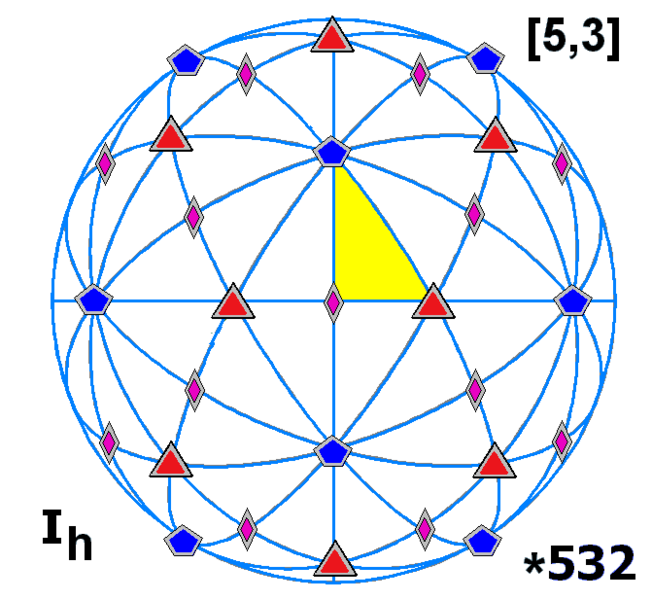
\includegraphics[scale = 0.75]{figures/symmetry.png}
        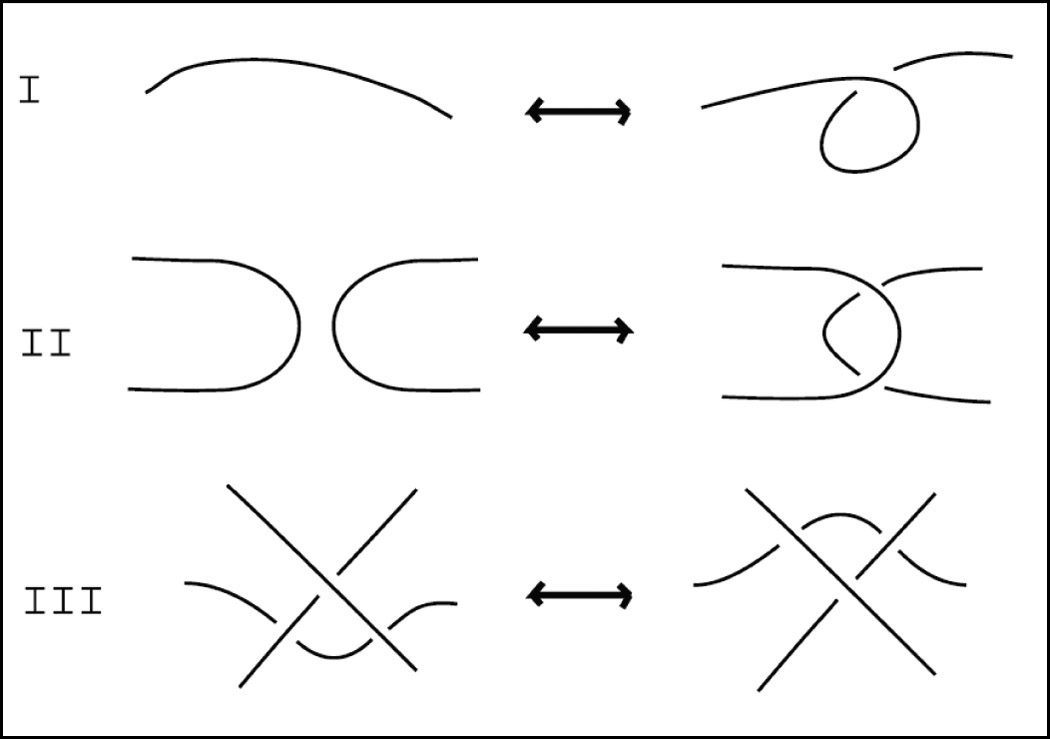
\includegraphics[scale = 0.75]{figures/reidemeisterMoves.jpg}


    \end{frame}

    \begin{frame}
        \frametitle{Background: History}
    \begin{itemize}
        \item Dr. Mizumitzu Takasaki was the first to investigate quandles. He was motivated by reflections in finite geometry. 

        \pause 

        \item Dr. Matveev and Dr. David Joyce independently discovered the \textbf{knot quandle}: a complete invariant up to orientation.

        \pause

    \item Matveev's formulation of the knot quandle was geometric, while David Joyce's was combinatorial.Both definitions are equivalent.

        \pause

    \item Quandles are a complete invariant, but hard to understand. This motivates the study of quandles as an algebraic theory in their own right. \cite{birrell2007knot}
    \end{itemize}
    \end{frame}

    \begin{frame}
        \frametitle{Background: Definition of a quandle}

        \begin{definition} \cite{birrell2007knot} \cite{joyce1982classifying}
            A quandle is a set $Q$, paired with operations $\thru$ and $\bthru$ such that the following axioms are satisfied:
        \end{definition}
        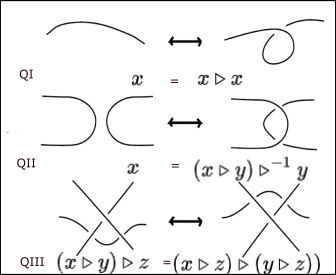
\includegraphics[scale = 0.75]{figures/reidemeisterMoves.png}
    \end{frame}

    \begin{frame}
        \frametitle{Background: Quandles and Groups}

        \begin{itemize}
            \item Quandles and groups are closely related.

            \pause

            \item Quandles are the algebraic theory of conjugation in groups.

            \pause

            \item Every conjugacy class $C_\alpha$ is a subquandle of $\Conj(G)$.
            \begin{definition}
            Every group $G$ gives rise to a quandle $\Conj(G)$, where the operation is $ g\thru h = \inv{h}gh $.
            \end{definition}

            \item The correspondence $G\mapsto \Conj(G)$ is the object function of a functor,
            \[
                \Conj:\mathbf{Quand} \to \mathbf{Grp}
                \]

        \end{itemize}

    \end{frame}

    \begin{frame}[fragile]
        \frametitle{Background: Adconj}

        \begin{theorem}\cite{joyce1982classifying}
        The functor $ \Conj:\mathbf{Grp} \to \mathbf{Quand} $ has a left adjoint (David Joyce).
        \end{theorem}

        \begin{definition}
            The universal augmentation group, $\Adconj(Q)$, is the group defined $ \Adconj(Q) = \langle x\in Q| x\thru y \inv{y}\inv{x}\inv{y};x,y\in Q \rangle $
            The correspondence $Q\mapsto \Adconj(Q)$ is the object function of a functor $\mathbf{Quand}\to \mathbf{Grp}$.
        \end{definition}
    \begin{theorem}
        $\Adconj$ is the left adjoint to $\Conj$.
        \[\begin{tikzcd}
            Q & \Conj(\Adconj(Q)) \\
            & \Conj(G)
            \arrow["\eta",from=1-1, to=1-2]
            \arrow["\phi"',from=1-1, to=2-2]
            \arrow["\Conj(\tilde{\phi})",dashed,from=1-2, to=2-2]
        \end{tikzcd}\]
    \end{theorem}

    \end{frame}



    \begin{frame}
        \frametitle[allowframebreaks]{Background: Significance of Adconj}

        There is geometric significance to the functor $\Adconj$.

        \begin{theorem}
            Let $K$ be a knot, and let $Q(K)$ be it's quandle. Then $ \Adconj(Q(K)) \cong \pi_1(S^3\setminus K)$. \cite{birrell2007knot}
        \end{theorem}

        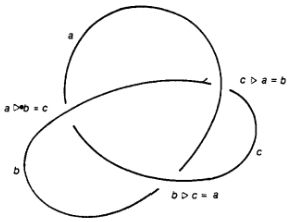
\includegraphics[scale = 1]{figures/taitQuandle.png}

        \begin{example}
        As an example, $ Q(K_3) $ is the quandle of transpositions of $S_3$ under conjugation. $ \Adconj(Q(K_3)) $ is the braid group on three strands.
        \end{example} \cite{wikipediaKnotGroup}
    \end{frame}

    \begin{frame}
    
        \frametitle{Background: Significance of Adconj}
        
        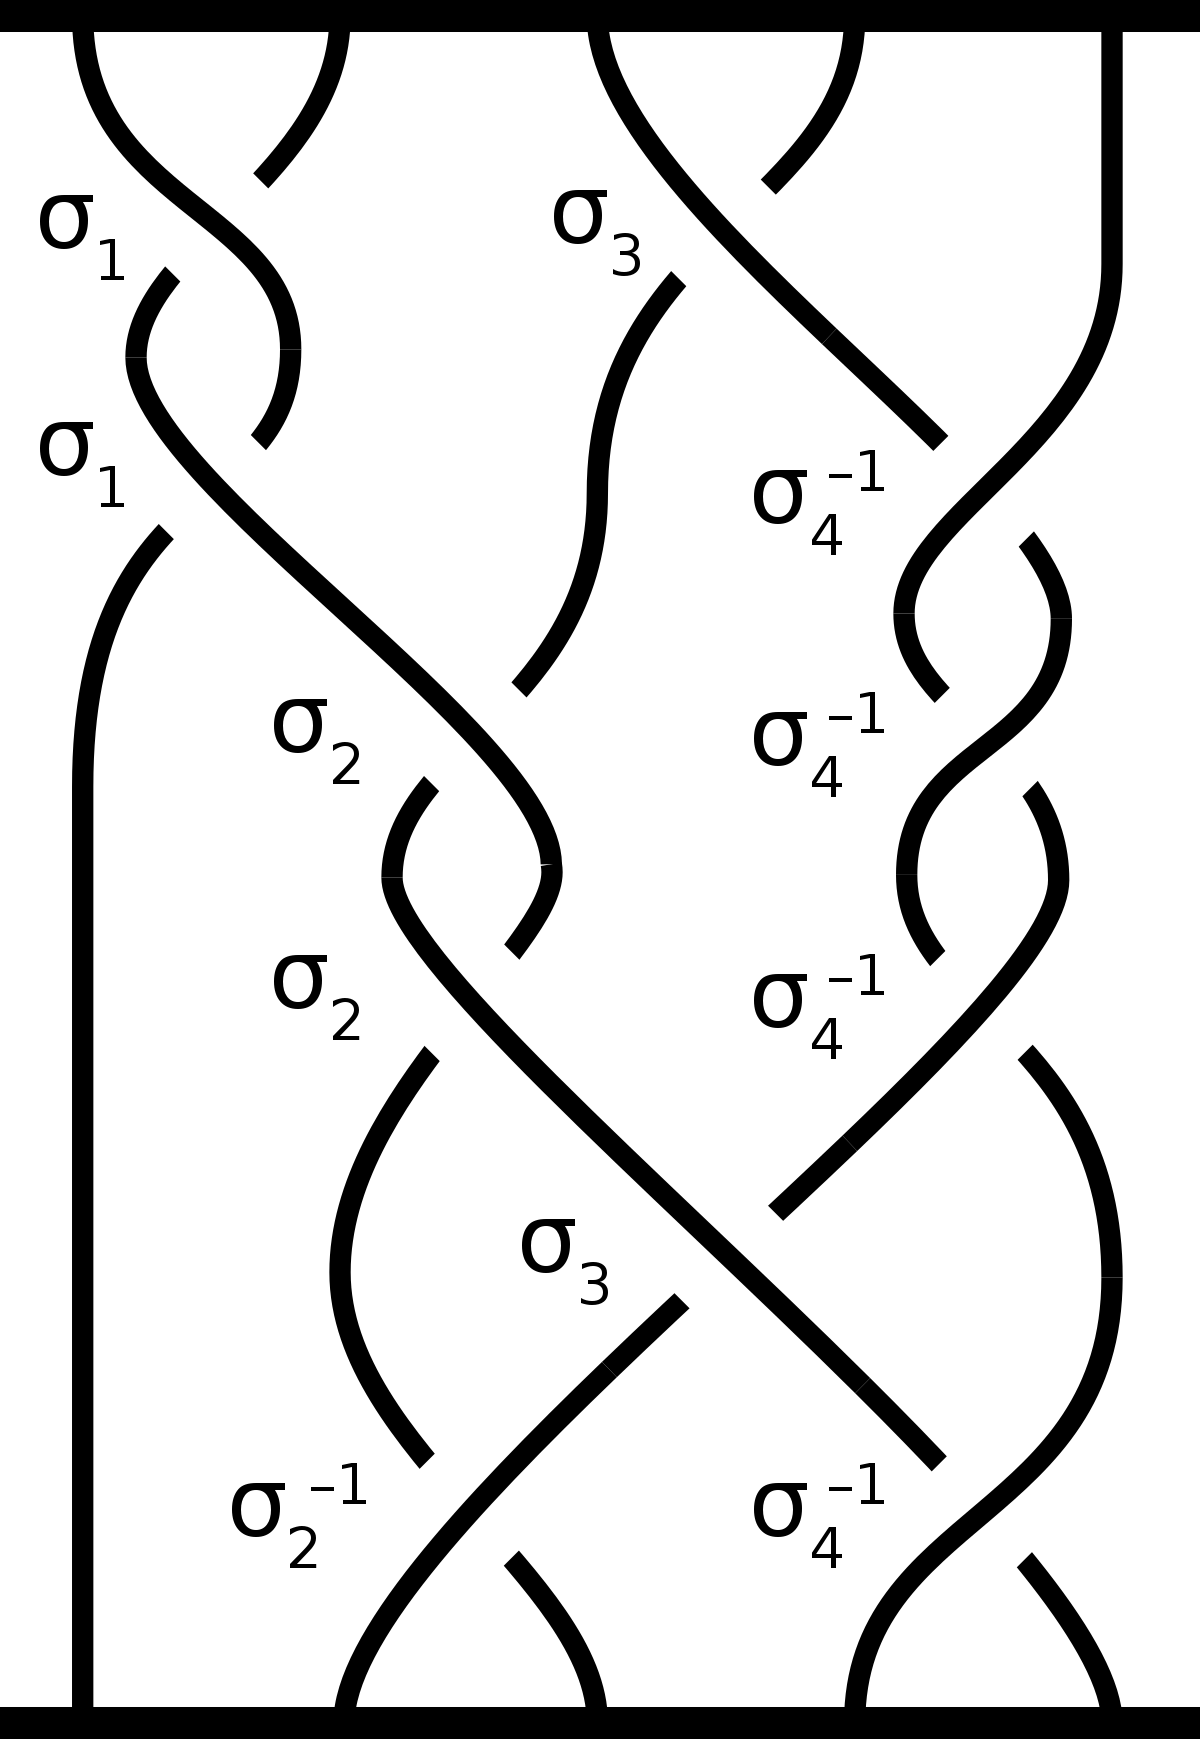
\includegraphics[scale = 0.1]{figures/braidGroup.png}

    \end{frame}

    \begin{frame}
        \frametitle{Takasaki Keis}

        \begin{definition}\cite{joyce1982classifying}
            A \textbf{kei} is a quandle $K$ whose operation is involutory: $ x\thru y \thru y = x $ for all $x,y\in K$.
        \end{definition}

        \begin{definition}
            Given any abelian group $A$, one can form a quandle, $\Tak(A)$, with operation $ x\thru y = 2y - x $. This is the object function of a functor,
            \[
                \mathbf{Kei}\to \mathbf{Ab}.
                \]
        \end{definition}

        We'll show that this functor has an adjoint. The Takasaki functor provides a lot of useful (counter)examples.

        
    \end{frame}


    \begin{frame}{Background: Semidisjoint Union}
        \begin{definition}\cite{ehrman2008toward}
        Given a sequence of quandles $Q_1, \dots , Q_n$ and a $nxn$ matrix of group homomorphisms $(M)_{ij} = g_{ij} : $, Ehrman et al. \cite{ehrman2008toward} defined the \textbf{semidisjoint union} as follows:
        \begin{align*}
            \#(Q_1, \dots, Q_n, M) = \Big(\coprod_{i = 1}^nQ_i, \thru\Big).
        \end{align*}
        \end{definition}
        \pause
        \begin{itemize}
            \item Each entry of the matrix $g_{ij}:\Adconj (Q_i)\to \Aut(Q_j)$ is a group homomorphism. 
            
            \item $\thru$ is defined as $x\thru y = x\cdot g_{ij}(|y|_{Q_i})$ for $x\in Q_i$ and $y\in Q_j$.
            
            \item Note that we are not guaranteed that the semidisjoint union is a quandle. If the matrix $M$ gives rise to a quandle, it is called a \textbf{mesh}.
            \item Ehrman et al. provided a necessary and sufficient condition for $M$ to be a mesh.
        \end{itemize}
        
    \end{frame}


    \begin{frame}
        \frametitle{Background: The Inner Automorphism Group}

        Probably the most important group (for our purposes) is the inner automorphism group.


    \begin{definition}
        An inner automorphism is a string of successive symmetries. The inner automorphism group is the group generated by the symmetries at elements, denoted $\Inn(Q) = <S(Q)>$.
        \end{definition}
        
        
        Warning! While the symmetries at elements are inner automorphisms, not all inner automorphisms are symmetries at elements. This is due to the fact that the quandle operation is \textbf{not} associative in general. 
        
    \end{frame}


    \begin{frame}{Background: Orbit Decomposition}

        \begin{theorem}<1->\cite{ehrman2008toward}
        Let $Q$ be a quandle, and let $Q_1,\dots, Q_n$ be its orbits under the inner automorphism group. Then we can construct a mesh $M$ such that 
        \[Q = \#(Q_1, \dots, Q_n, M).\]
        \end{theorem}
        \vspace{0.15in}
        \begin{itemize}
        
            \item<2-> Note that the orbits need not be connected. Hence the orbits themselves may be decomposable via the previous theorem. 
        
        \end{itemize}
        
            
        \end{frame}

        
    \begin{frame}{Subquandle Lattices}

        \begin{definition}
        The set of subquandles of any quandle $Q$ under inclusion forms a lattice \cite{saki2021complemented}, which we denote as $\cL(Q)$. 
        \end{definition}
        \pause
        
        \begin{definition}
        Given two subquandles $Q_1, Q_2\sq Q$, their \textbf{meet} is $Q_1\wedge Q_2 = Q_1\cap Q_2$ and their \textbf{join} is $Q_1\vee Q_2 =  \qgen{Q_1\cup Q_2}$.
        \end{definition}
        \pause
        
        \begin{definition}
        A subquandle $Q_1\sq Q$ is \textbf{complemented} in $Q$ if there is some $Q_2\sq Q$ such that $Q_1 \wedge Q_2 = \emptyset$, and $Q_1\vee Q_2 = Q$. The subquandle lattice $\cL(Q)$ is complemented if every subquandle is complemented.
        \end{definition}
    \end{frame}

    \begin{frame}
        \frametitle{Subquandle Lattices}
        Just as with groups and other algebraic structures, subquandle lattices can be visualized by an inclusion diagram. 
        
        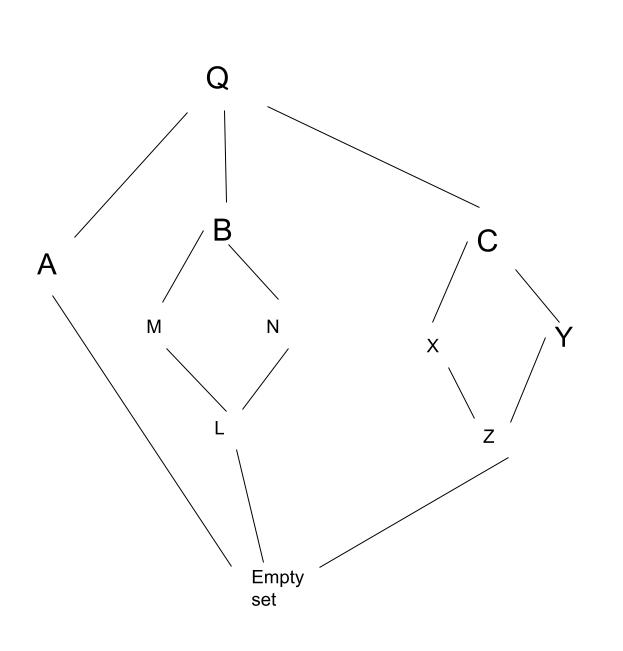
\includegraphics[scale = 0.2]{figures/sqlattice.jpg}
    \end{frame}
    
\begin{frame}{Two Actions}

    \begin{itemize}
        \item We've shown how $\Inn(Q)$ acts on $Q$ by functional application.
        \item This action allows us to construct an action of $\Inn(Q)$ upon $\mathcal{L}(Q)$.
    \end{itemize}
    
    \vspace{0.5cm}
    \begin{definition}
    The action of $\Inn (Q)$ on Q' is also given by functional application, denoted $Q'\cdot \Inn(Q)$. \\
    \vspace{0.15in}
    The action of $\Inn(Q)$ upon $\mathcal{L}(Q)$ is defined $Q'\sigma = \sigma(Q')$ for all $Q'\in \mathcal{L}(Q)$, and for all $\sigma\in \Inn(Q)$.
    The orbit of $Q'$ under this action is denoted by $[Q']\cdot \Inn(Q) = \{ Q'\sigma: \sigma \in \Inn(Q)\}$.\\
    \end{definition}
    \end{frame}


    \begin{frame}{Two Actions}
        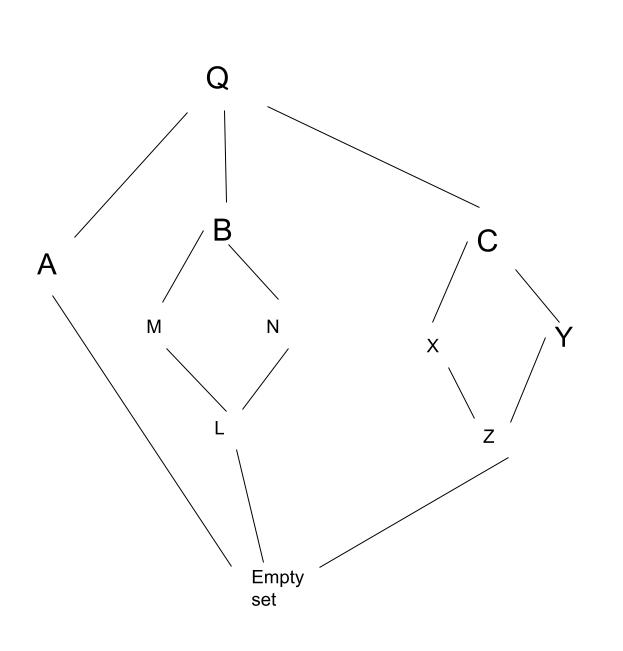
\includegraphics[scale = 0.35]{figures/sqlattice.jpg}
        \end{frame}
        
        \begin{frame}{Acting on the subquandle lattice}
        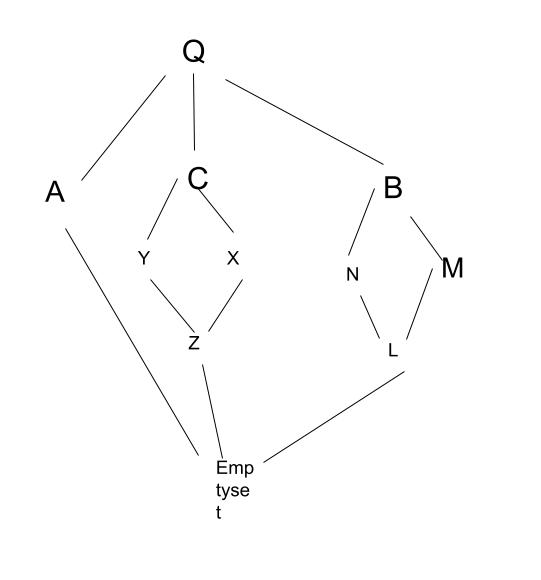
\includegraphics[scale = 0.35]{figures/other_sqlattice.jpg}
        \end{frame}
        
        \begin{frame}{Acting on the subquandle lattice}
        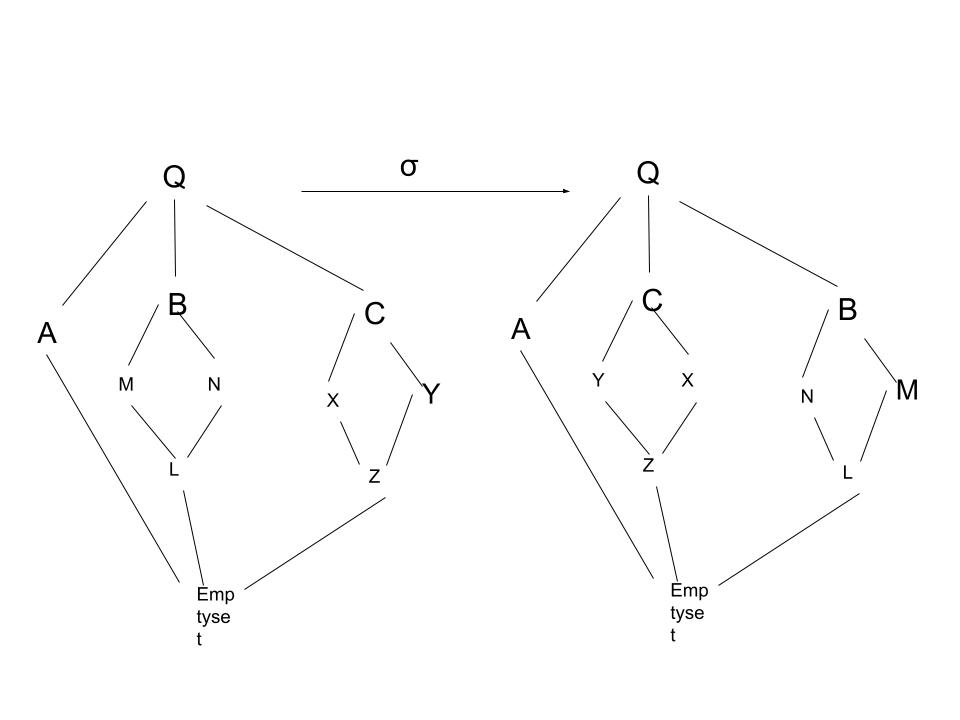
\includegraphics[scale = 0.35]{figures/lattice_transformation.jpg}
    \end{frame}


    \begin{frame}{Background: Saki And Kiani's Paper}

        Saki and Kiani showed that the subrack lattice of a finite rack is complemented. Since quandles are racks, this holds for quandles as a corollary.
        
        \begin{corollary}
        The subquandle lattice of every finite quandle is complemented.
        \end{corollary}
        \vspace{0.2in}
        \pause
        
        \begin{theorem}[Saki and Kiani]
        Consider the quandle $\Q$ with the dihedral structure, $x\thru^* y = 2x-y$, $\forall x,y\in \Q$. The subquandle $\{0\}$ is not complemented.
        \end{theorem}
    \end{frame}

    
    \begin{frame}
        \frametitle{Equivalence Theorem}
        \begin{theorem}
            \label{equivalenceTheorem}
            Let $Q$ be a quandle, and let $Q'\sq Q$. Denote the subquandle lattice of $Q$ by $\mathcal{L}(Q)$. The following are equivalent:
            \begin{enumerate}
                \item $Q\setminus Q'\sq Q$,
                \item $Q'$ is a union of orbits under the action of $\Inn(Q)$ on $Q$,
                \item $Q'$ is a fixed point of the action of $\Inn(Q)$ on $\mathcal{L}(Q)$,
                \item $Q = \#(Q',Q\setminus Q', M)$ for a mesh $M$.
            \end{enumerate}
        \end{theorem}
    \end{frame}


\begin{frame}{Strongly Complemented Within Strongly Complemented}


    \begin{lemma}[1]
    Let $Q''\sq Q' \sq Q$ such that $Q''$ is strongly complemented within $Q'$, and $Q'$ is strongly complemented within $Q$. Then for any $\gamma\in \Inn(Q)$, $Q''\gamma$ is strongly complemented within $Q'$.
    \end{lemma}
    \pause
    \begin{lemma}[2]
    Let $Q''\sq Q' \sq Q$ be as in Lemma (1). Then for all $\sigma\in \Inn(Q)$, there exists some $\sigma'\in \langle S(Q\setminus Q')\rangle$ such that $Q''\sigma = Q''\sigma'$.
    \end{lemma}
    \begin{proof}
    \begin{itemize}
        \item Suppose $\sigma = S_{x_1}^{\epsilon_1}\dots S_{x_n}^{\epsilon_n}$ for each $x_j\in Q$, $\epsilon_j \in \{-1,1\}$.
        \item Suppose $\exists x_i \in Q'$ whose symmetry appears in $\sigma$ which we cannot remove without changing the action.
        \item By Lemma 1, $Q''$ acted upon by the string of $\sigma$ up until $x_i$, denote it by $\gamma$, is strongly complemented in $Q'$.
    \end{itemize}
    \end{proof}
    \end{frame}

    \begin{frame}
        \frametitle{Strongly Complimented Subquandles}

        Our research centered around revealing finer structure to the ways in which subquandle 
        fit within the subquandle lattice.
    \end{frame}


    \begin{frame}{Strongly Complemented Within Strongly Complemented}

        \begin{proof}[Proof (\textit{continued})]
        
        \begin{itemize}
            \item Since $x_i\in Q'$, $S_{x_i}|_{Q'}$ acts the same upon $Q'$ as $S_{x_i}$
            \item Then, $Q''\gamma S_{x_i} = Q''\gamma$ by the equivalence theorem. Hence, removing $S_{x_i}$ won't change anything, so there never was a counterexample.
            \item Thus, we can construct $\sigma'$ by removing symmetries represented by elements in $Q'$.
        \end{itemize}
         
        \end{proof}
        
        
        \begin{lemma}[3]
        
        Suppose that $Q''$ is strongly complemented within $Q$, while $Q''\sq Q'\sq Q$. Then, $Q''$ is strongly complemented within $Q'$.
        
        \end{lemma}
        
        \end{frame}
        
        \begin{frame}{Strongly Complemented Within Strongly Complemented}
        
        \begin{theorem}
        Suppose $Q$ is a quandle, with subquandles $Q''\sq Q'\sq Q$, such that $Q''$ is strongly complemented within $Q'$, while $Q'$ is strongly complemented within $Q$. Then $Q''$ is complemented within $Q$ by the subquandle $Q\setminus Q''\cdot \Inn(Q)$.
        \end{theorem}
        \pause
        
        \begin{proof}
        \begin{itemize}
            \item By Lemma 3 and the equivalence theorem, $Q''$ is strongly complemented within $Q''\cdot \Inn(Q)$, which in turn is strongly complemented within $Q$.
            \item $Q''\wedge Q\setminus Q''\cdot \Inn(Q) = \emptyset$
            \item Using Lemmas 2 and 1, we show that $Q''\cdot \Inn(Q) \subset Q''\vee Q\setminus Q''\cdot \Inn(Q)$, hence $Q''\vee Q\setminus Q''\cdot \Inn(Q) = Q$.
            \item Hence $Q''$ has $Q\setminus Q''\cdot \Inn(Q)$ as a complement.
        \end{itemize}
        \end{proof}
            
        \end{frame}

\begin{frame}
    \frametitle{possible extensions of Saki and Kiani's results}

    \begin{itemize}
        \item 
        \begin{question}
            Do ind-finite quandles have complimented sublattices?
        \end{question}
        \pause
        \item 
        \begin{question}
            Do pro-finite quandles have complimented sublattices?
        \end{question}

    \end{itemize}
\end{frame}
    
\begin{frame}{Ind-finite Quandles}
    % Investigate whether Saki and Kiani's results about finite quandles specializes to certain classes of infinite quandles that are more similar to finite quandles: ind-finite quandles and profinite quandles.
    Although ind-finite objects are generally defined in terms of direct limits, a less abstract definition is available with quandles.
    \begin{definition}
    A nonempty quandle $Q$ is \textbf{ind-finite} if there is a family of finite subquandles $\{Q_i\}_{i \in \cI}$ indexed by a directed set $\cI$ such that each $Q_i\sq Q$, $|Q_i|<\infty$, $Q_i\psq Q_{i+1}$, and $Q=\bigcup_{i\in\cI} Q_i.$ 
    \end{definition}    
    \pause
    
    \begin{lemma}
    Suppose $Q$ is a quandle. Then, $Q$ is ind-finite if and only if every finitely generated subquandle of $Q$ is finite.
    \end{lemma}
    \pause
    
    \begin{example}
    Let the quandle operation $\thru^*$ be given by $x\thru^* y = 2x-y$.\\
    \begin{itemize}
    \item Neither $(\Q,\thru^*)$ nor $(\Q/\Z,\thru^*)$ has a complemented sublattice.
    \item $(\Q / \Z, \thru^*)$ is ind-finite but $(\Q, \thru^*)$ is not.
    \end{itemize}
    \end{example}

    This answers our first question: no!
\end{frame}
    


\begin{frame}[fragile]
    \frametitle{Background: Adconj}
    The functor $ \Conj:\mathbf{Grp} \to \mathbf{Quand} $ has a left adjoint (David Joyce).

    \begin{definition}
        Given a directed set $\mathcal{I}$, an inverse system of quandles is a family of quandles $ Q_i $ for $i\in \mathcal{I}$, and a family of quandle homomorphisms $ \phi_{ij}:Q_i\to Q_j $ for $i\le j$,
        such that for all $i\le j\le k$, we have a commutative diagram

        The limit of this diagram (which always exists for quandles), is the inverse limit of such an inverse system.
        \[\begin{tikzcd}
            Q_i & Q_j \\
            & Q_k
            \arrow["\phi_{ij}", from=1-1, to=1-2]
            \arrow["\phi_{ik}"', from = 1-1, to=2-2]
            \arrow["\phi_{jk}", from=1-2, to=2-2]
        \end{tikzcd}.\]
        A \textbf{profinite quandle} is the limit of an inverse system.
    \end{definition}

    
    \pause

    \begin{remark}
        As you might guess, these are a lot harder to think about. 
    \end{remark}

\end{frame}



    \begin{frame}
        \frametitle{Limit Preserving Functors}

        One useful way of finding functors that 1) preserve limits, and 2) send finite objects to finite objects.

        \begin{definition}
            A functor $F:\mathcal{C}\to \mathcal{D}$  is a right adjoint if there is another functor $ G:\mathcal{D}\to \mathcal{C} $ such that for any object $c\in \mathcal{C}$, there is a morphism $\eta : c\to G(F(c)) $
        \end{definition}

        \begin{theorem}
            A functor $F:\mathcal{C}\to \mathcal{D}$ (where $\mathcal{C}$ and $\mathcal{D}$ are complete) preserves limits if it has a right adjoint.
        \end{theorem}
    \end{frame}

    \begin{frame}
        \frametitle{Profinite Quandles and the Takasaki Functor}
        \begin{theorem}
            The functor $\Tak : \mathbf{Ab} \to \mathbf{Kei}$ is a right adjoint, with left adjoint $ \Adtak:\mathbf{Kei} \to \mathbf{Ab} $, with object function 
            \[K \mapsto \langle x\in K \rangle_{\mathbf{Ab}} / \langle(x\thru y - 2y + x: x,y\in K)\rangle_{\mathbf{Ab}} \]
        \end{theorem}

        
        \begin{corollary}
            For any profinite abelian group $A$, $ \Adtak(A) $ is a profinite quandle.
        \end{corollary}

    \end{frame}

    \begin{frame}
        \frametitle{Some Examples of Profinite Quandles}

        \begin{example}
            $Tak(A)$ for any profinite abelian group. In particular, $\Tak(\Z_p)$ for any prime $p$.
        \end{example}

        \begin{example}
            $ \Conj(G) $ for any profninite group $G$ (we already know $\Conj$ is a right adjiont).
        \end{example}
    \end{frame}

    \begin{frame}
        \frametitle{Open Questions}

        \begin{question}
            Do profinite quandles have complimented sublattices?
        \end{question}

        \begin{question}
            Can the partial transitivity condition be extended?
        \end{question}

        \begin{question}
            Can we find an example in which the partial transitivity condition holds non-trivially?
        \end{question}
    \end{frame}

    \begin{frame}[allowframebreaks]{bib}
        \printbibliography
    \end{frame}

\end{document}
